\documentclass[UTF8]{ctexart}
\usepackage[colorlinks=true]{hyperref}

\usepackage{amsmath, bm,amsfonts}
\usepackage{hyperref}
\usepackage[normalem]{ulem}
% \usepackage{enumitem}
% \setlist{nosep}
\usepackage{caption}
\usepackage{graphicx}
% \graphicspath{{./pic/}}
\usepackage[usenames, dvipsnames]{xcolor}
\usepackage{listings}
% settings for listings.sty
\renewcommand{\lstlistingname}{代码清单}
\lstdefinestyle{lfonts}{
  basicstyle   = \footnotesize\ttfamily,
  stringstyle  = \color{purple},
  keywordstyle = \color{blue!60!black}\bfseries,
  commentstyle = \color{olive}\scshape,
}
\lstdefinestyle{lnumbers}{
  numbers     = left,
  numberstyle = \tiny,
  numbersep   = 1em,
  firstnumber = 1,
  stepnumber  = 1,
}
\lstdefinestyle{llayout}{
  breaklines       = true,
  tabsize          = 2,
  columns          = flexible,
}
\lstdefinestyle{lgeometry}{
  xleftmargin      = 15pt,
  xrightmargin     = 0pt,
  frame            = tb,
  framesep         = \fboxsep,
  framexleftmargin = 15pt,
}
\lstdefinestyle{lgeneral}{
  style = lfonts,
  style = lnumbers,
  style = llayout,
  style = lgeometry,
}
\def\beginlstdelim#1#2#3{%
  \def\endlstdelim{#2\egroup}%
  \ttfamily#1\bgroup\color{#3}\aftergroup\endlstdelim}
\lstdefinestyle{ldelims}{
  moredelim = **[is][\beginlstdelim{\$}{\$}{orange}]{\$}{\$},
  moredelim = **[is][\beginlstdelim{\{}{\}}{ForestGreen}]{\{}{\}},
  moredelim = **[is][\beginlstdelim{[}{]}{cyan}]{[}{]},
}
% LaTeX lst style
\lstdefinestyle{lltx}{
  language = {[LaTeX]TeX},
  style = lgeneral,
  style = ldelims,
  morekeywords = {% LaTeX original commands
    maketitle,
    rmfamily, sffamily, ttfamily,
    itshape, slshape, scshape,
    mdseries, bfseries, emph,
    textrm, textsf, texttt,
    textit, textsl, textsc,
    textmd, textbf,
    newcommand, renewcommand, providecommand,
    cs, meta, marg, oarg, parg
  }
}
\lstdefinestyle{iltx}{
  style      = lltx,
  basicstyle = \ttfamily
}
\lstdefinestyle{lbash}{
  language   = {bash},
  style      = lgeneral,
}
\lstdefinestyle{ibash}{
  style      = lbash,
  basicstyle = \ttfamily
}

% code style setting
\definecolor{codegreen}{rgb}{0,0.6,0}
\definecolor{codegray}{rgb}{0.5,0.5,0.5}
\definecolor{codepurple}{rgb}{0.58,0,0.82}
\definecolor{backcolour}{rgb}{0.95,0.95,0.92}

\lstdefinestyle{mystyle}{
	backgroundcolor=\color{backcolour},   
	commentstyle=\color{codegreen},
	keywordstyle=\color{magenta},
	numberstyle=\tiny\color{codegray},
	stringstyle=\color{codepurple},
	basicstyle=\footnotesize,
	breakatwhitespace=false,         
	breaklines=true,                 
	captionpos=b,                    
	keepspaces=true,                 
	numbers=left,                    
	numbersep=5pt,                  
	showspaces=false,                
	showstringspaces=false,
	showtabs=false,                  
	tabsize=2
}
\endinput

\usepackage{hologo}
\usepackage{subfigure}
\usepackage{changepage}

\ctexset{
    section = {
        titleformat = \raggedright,
        name = {第,节},
        number = \chinese{section}
    }
}

\title{mmdetection解析}
\author{Sisyphes,yehao}
\date{2019年8月1日}

\begin{document}
\maketitle
\tableofcontents
\newpage

% \include{lang-natural}
% \include{lang-computer}
% \section{已有资源}
% \href{https://heary.cn/}{基于PyTorch的开源目标检测系统},
% \href{https://nicehuster.github.io/2019/04/08/mmdetection/}{mmdetection解析},
% \href{https://blog.csdn.net/weicao1990/article/details/95332938}{mmdetection源码阅读笔记},
% \href{http://spytensor.com/index.php/archives/53/}{奇淫技巧}.
\section{结构设计}
\begin{itemize}
	\item BackBone:特征提取骨架网络,ResNet,ResneXt等.
	\item Neck: 连接骨架和头部.多层级特征融合,FPN,BFP等.
	\item DenseHead:处理特征图上的密集框部分, 主要分AnchorHead, AnchorFreeHead两大类,分别有RPNHead, SSDHead,RetinaHead和FCOSHead等.
	\item RoIExtractor:汇集不同层级的特征框,将其大小统一,为二步定位,类别优化服务.
	\item RoIHead (BBoxHead/MaskHead):类别分类或位置回归等.
	\item OneStage: BackBone + Neck + DenseHead
	\item TwoStage: BackBone + Neck  + (DenseHead) + RoIExtractor + RoIHead
	
\end{itemize}


\noindent 代码结构:\\
configs 网络组件结构等配置信息\\
tools:训练和测试的最终包装\\
mmdet:
\begin{adjustwidth}{0.5cm}{0cm}
	apis: 分布式环境设定,推断和训练基类代码\\
	core: anchor,bbox,mask等在训练前和训练中的各种变换函数\\
	datasets:coco和voc格式的数据类以及一些增强代码\\
	models:模型组件,采用注册和组合构建的形式完成模型搭建\\
	ops:优化加速代码,包括nms,roialign,dcn,gcb,mask,focal\_loss等\\
\end{adjustwidth}

\begin{figure}[htbp]
	\centering
	\begin{minipage}[t]{0.48\textwidth}
	\centering
	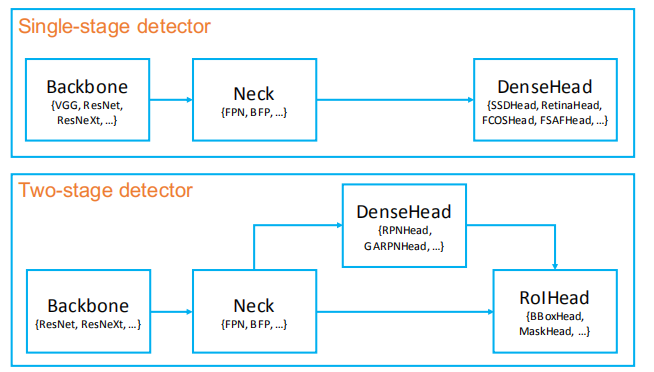
\includegraphics[width=5cm, height=3cm]{./pic/mmdetect.png}
	\caption{ Framework }
	\end{minipage}
	\begin{minipage}[t]{0.48\textwidth}
	\centering
	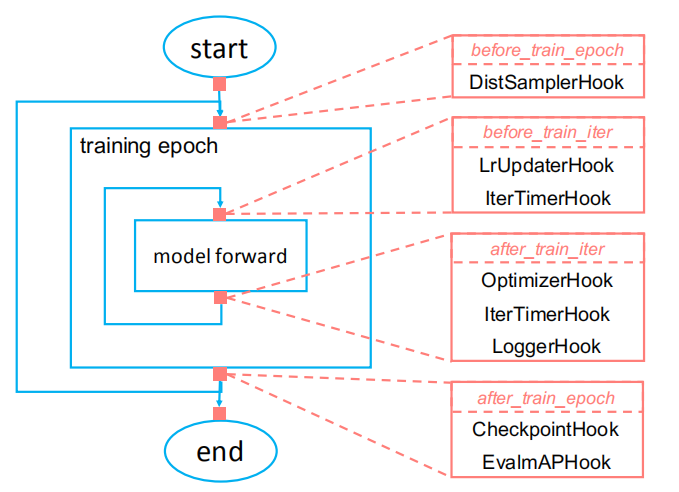
\includegraphics[width=5cm,height=3cm]{./pic/mmdetect_pipe.png}
	\caption{Trainning pipeline}
	\label{trainpipe_pic}
	\end{minipage}
\end{figure}

% \newpage
\subsection{总体逻辑}
在最外层的train.py中能看到:\\
1. mmcv.Config.fromfile从配置文件解析配置信息,并做适当更新,包括预加载模型文件,分布式相关等\\
2. mmdet.models.builder 中的build\_detector根据配置信息构造模型

\begin{adjustwidth}{0.5cm}{0cm}

2.5 build函数调用\_build\_module(新版为build\_from\_cfg)函数,按type关键字从注册表中获取相应的
模型对象,并根据配置参数实例化对象(配置文件的模型参数只占了各模型构造参数的一小部分,模型结构并非可以随意更改).\\
2.6 registr.py实现了模型的注册装饰器,其主要功能就是将各模型组件类对象保存到registry.module\_dict中,从而可以实现2.5所示功能.\\
2.7 目前包含BACKBONES,NECKS,ROI\_EXTRACTORS,SHARED\_\\
HEADS,HEADS,LOSSES,DETECTORS七个(容器).注册器可按@N
AME.register\_module方式装饰,新增.所有被注册的对象都是一个完整的pytorch构图\\
2.9 @DETECTORS.register\_module装饰了完整的检测算法(OneStage,TwoStage),各个部件在其init()函数中实例化,实现2.5的依次调用.
\end{adjustwidth}
3. 最后是数据迭代器和训练pipeline\ref{trainpipeline}.

\subsection{Configs}
配置方式支持python/json/yaml,从mmcv的Config解析,其功能同maskrcnn-benchmark的yacs类似,将字典的取值方式属性化.

配置文件模型部分包含模型组件及其可改动模型结构的参数,比如backbone的层数,冻结的stage;bbox\_head的in\_channel,类别,损失函数等;训练部分主要包括anchor采样相关系数;测试包括非极大抑制等相关参数;剩下数据,优化器,模型管理,日志等相关信息,一看即明.

\newpage
\subsection{Backbone}
\label{backbone}

\begin{figure}[htbp]
	\centering
	\begin{minipage}[t]{0.48\textwidth}
	\centering
	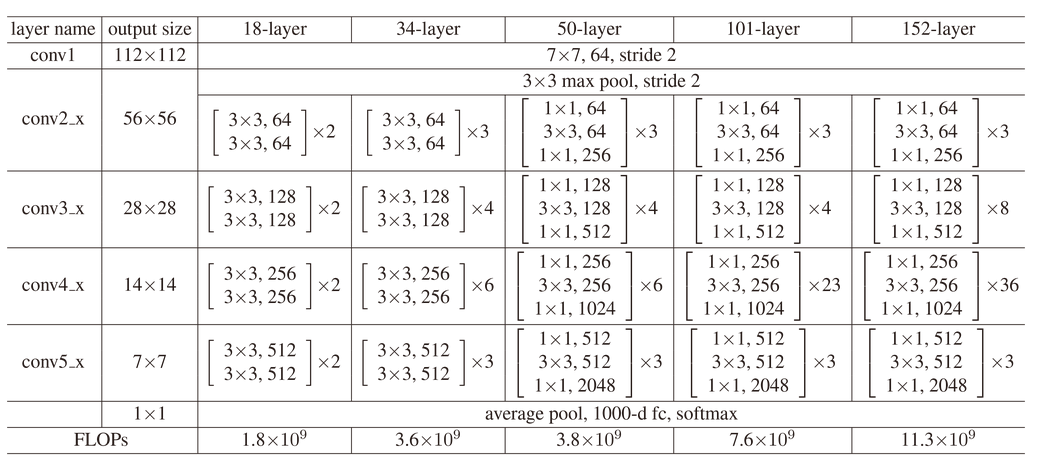
\includegraphics[width=5cm, height=4cm]{./pic/resnet_struct.png}
	\caption{resnet}
	\label{picresnet}
	\end{minipage}
	\begin{minipage}[t]{0.48\textwidth}
		\centering
		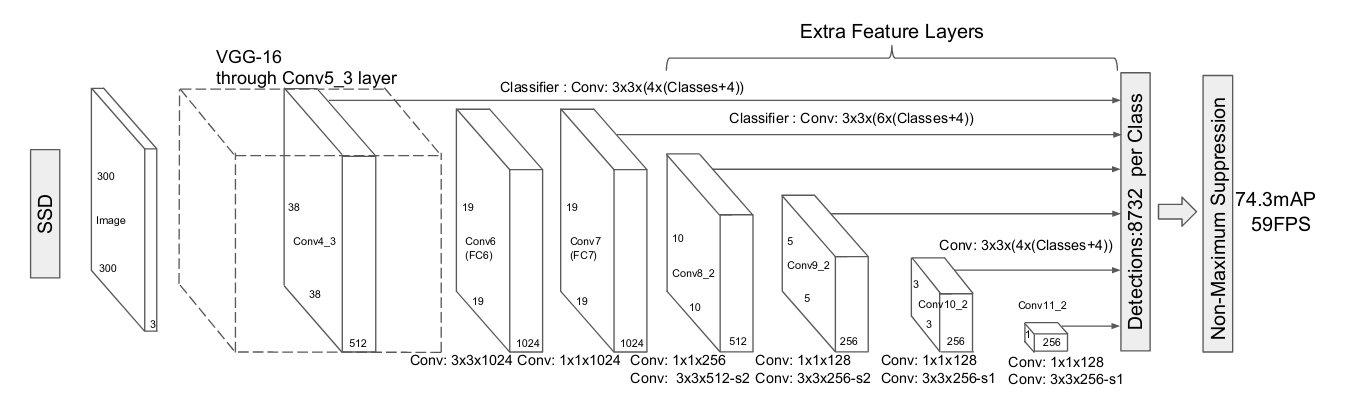
\includegraphics[width=5cm,height=4cm]{./pic/ssd.png}
		\caption{ssd}
		\label{picssd}
	\end{minipage}
\end{figure}

% \begin{figure}[htbp]
% 	\centering
% 	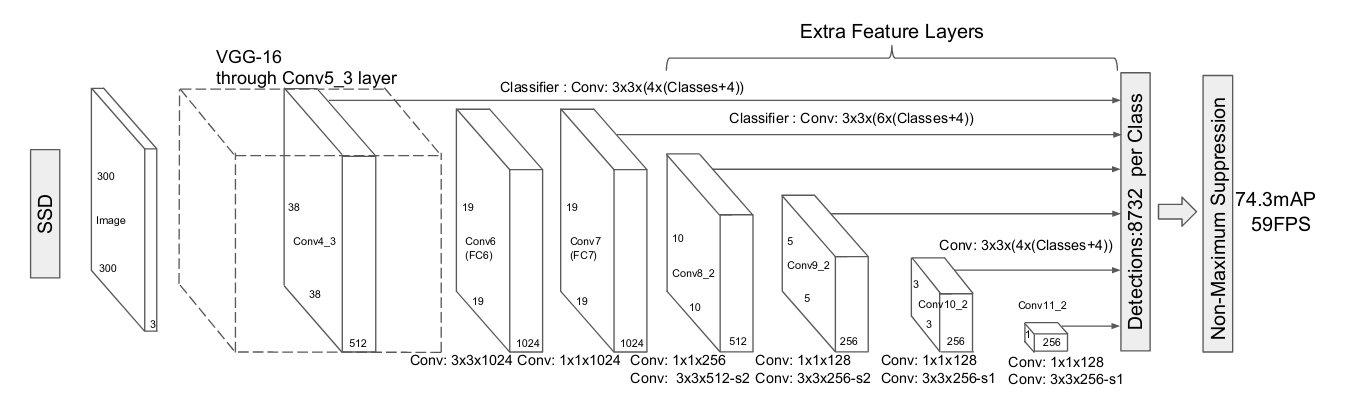
\includegraphics[width=5cm, height=4cm]{./pic/ssd.png}
% 	\caption{config maskrcnn}
% \end{figure}


\subsection{Necks}
\begin{figure}[htbp]
	\centering
	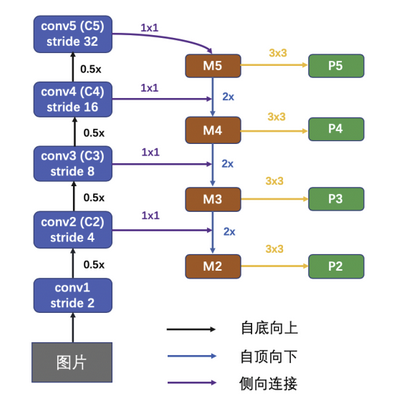
\includegraphics[width=5cm,height=4cm]{./pic/fpn.png}
	\caption{fpn}
	\label{picfpn}
\end{figure}
展开描述:目标尺度和金字塔层级的关系,这些层级对应的尺度与损失函数,样本采样等的关系.
% 要检测到$15\times15$的小目标,有哪些考虑点
\subsection{Heads}
anchor\_heads, bbox\_heads, mask\_heads都将有loss的计算,是核心点,需详细描述.

\subsubsection{ssdhead}
ssd结构的检测网络,目前已有ssd300,ssd512,结构细节参考\ref{backbone}. 从配置文件中可有看到,它没有neck,
因层级结构在backbone实现.

ssdhead继承自anchorhead,主要功能为处理多层级特征上的anchor构造和target标定与筛选,
基本的feauturemap上的acnhor生成由mmdet.core.
anchor中的AnchorGenerator完成,优化目标anchor由anhor\_target完成.
ssdhead中forward前向返回各层级对应的类别分数和坐标信息,loss函数则得到对应的损失函数,以字典的形式返回,最终求导时,汇总成一个值,同时也能计算各个部分损失函数的均值,方差,方便优化,debug.

此处的难点在于anchor的设定和target的标定,筛选.现就anchor这一块细说如下:

anchor基本介绍: anchor设计和caffe ssd anchor设计一致, 假设min\_size为$a$, max\_size为$b$, 则先生成ratio为1, 宽度和高度为$(a, a), (\sqrt{ab}$, 
$\sqrt{ab})$的两个anchor, ratio为$2, 1/2, 3, 1/3$则分别生成宽度和高度为$(a*\sqrt{ratio}, a/\sqrt{ratio})$的anchor, mmdetection中必须设定每一层的min\_size, max\_size, 因此ratios为$[2]$则对应4个anchor, ratios为$[2,3]$则对应6个anchor.

在init()函数中,先生成min\_size, max\_size, 注意它这里是必须要指定max\_size(和caffe SSD不同,无法生成奇数个anchor), 确保len(min\_size)=
len(max\_size), 调用AnchorGenerator()类生成了base\_anchors, 数量是6或者10,使用indices操作从6个anchor里选择$(0, 3, 1, 2)$或者从10个anchor里选择$(0, 5, 1, 2, 3, 4) $$\rightarrow$ 最终生成4个或者6个anchor.于在多个feature map上生成anchor,因此使用了一个for循环操作, 将anchor\_generator放入到anchor\_generatos[]中.


AnchorGenerator类, init()函数需要如下参数:

\begin{itemize}
	\item base\_size: 即设置的min\_size
	\item scales: 是$(1, \sqrt{max\_size / min\_size})$, 用来生成ratio为1的两个anchor
	\item ratios: 是$(1, 2, 1/2)$或者$(1, 2, 1/2, 3, 1/3)$
	\item ctr: ctr由stride生成, 是anchor的中心坐标, $(\frac{stride - 1}{2}, \frac{stride - 1}{2} ) $在gen\_base\_anchor()函数里, 使用上面的参数来计算base\_anchor, 计算流程如下:
	\begin{itemize}
		\item 根据ratios来计算h\_ratios和w\_ratios, 即上面所述的$(1 / \sqrt{ratios}$, $\sqrt{ratios}) $.
		\item 根据scales来计算base\_size, 一共有2个分别是$$(min\_size, \sqrt{min\_size * max\_size}) = min\_size * scales$$
		\item 计算anchors的宽度和高度, 只以宽度举例: $w = base\_size * w\_ratios$, 以ratios是$(1, 2, 1/2)$举例, base\_size shape为$(2, 1)$, w\_ratios shape为$(1, 3)$, 
		计算出的w是$(2, 3) $一共生成了6个anchor, 如果ratios是$(1, 2, 1/2, 3, 1/3)$, 则生成10个anchor (此处anchor数量和标准ssd anchor数量不一致 $\rightarrow$
		 再筛选(即ssd\_head.py中使用indices操作进行筛选))
	\end{itemize}
	
\end{itemize}

\subsection{Losses}
CrossEntropyLoss, SmoothL1Loss,Fcoalloss, BalancedL1Loss, IoULoss,
BoundedIoULoss, ArcLoss


\subsection{Detectors}
OneStage, TwoStage和能改动的地方.

\subsubsection{maskrcnn}
以配置文件mask\_rcnn\_r50\_fpn\_1x.py为例说说twao\_stage的实现过程.
配合two\_stage的forward\_train()函数和配置文件,即可.

首先backbone为resnet50,(resnet系列结构参见\ref{picresnet}),
其以tuple形式返回4个stage的特征图,片段代码如下:
% \begin{figure}[htbp]
% 	\centering
% 	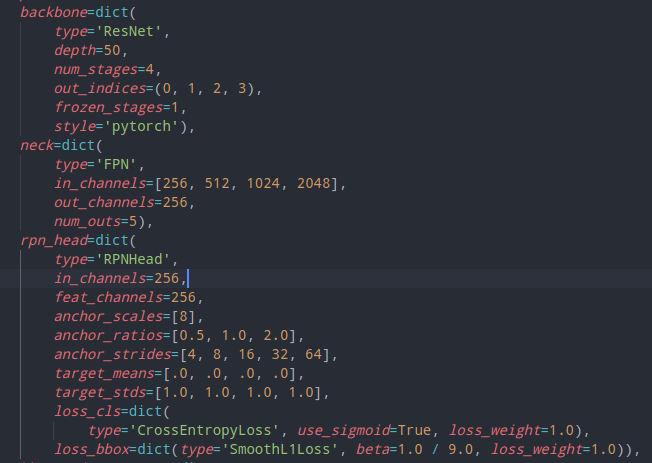
\includegraphics[width=5cm, height=4cm]{./pic/maskrcnn_50.png}
% 	\caption{config maskrcnn}
% \end{figure}
\lstset{style=mystyle}
\begin{lstlisting}[language=Python]

outs = []
for i, layer_name in enumerate(self.res_layers):
	res_layer = getattr(self, layer_name)
	x = res_layer(x)
	if i in self.out_indices:
		outs.append(x)

\end{lstlisting}

然后neck为fpn,结构参见\ref{picfpn},
fpn根据config中的out\_indices取出以resnet50输出的对应stage,分别构造输出channel维度统一的卷积算子,然后按照\ref{picfpn}所示融合方式进行不同尺度的特征融合,以元组形式输出结果.
在配置信息里有一条num\_outs=5,是为mask-rcnn在最顶层特征增加的最大池化特征输出.以上两块为提取特征,被extract\_feat整合在一块,

% \lstset{style=mystyle}
% \begin{lstlisting}[language=Python]
% 	for i in range(self.start_level, self.backbone_end_level):
% 		l_conv = ConvModule(
% 			in_channels[i],
% 			out_channels,
% 			1,
% 			conv_cfg=conv_cfg,
% 			norm_cfg=norm_cfg,
% 			activation=self.activation,
% 			inplace=False)
% 		fpn_conv = ConvModule(
% 			out_channels,
% 			out_channels,
% 			3,
% 			padding=1,
% 			conv_cfg=conv_cfg,
% 			norm_cfg=norm_cfg,
% 			activation=self.activation,
% 			inplace=False)

% 		self.lateral_convs.append(l_conv)
% 		self.fpn_convs.append(fpn_conv)

% \end{lstlisting}
紧接着forward\_train中包含了剩下的所有流程.
\begin{equation*}
	\begin{aligned}
		 rpn\_head \rightarrow rpn\_head.loss \rightarrow rpn\_head.get\_bboxes \rightarrow assign \rightarrow sample \\
		\rightarrow bbox\_roi\_extractor \rightarrow  bbox\_head \rightarrow bbox\_head.get\_target. \rightarrow bbox\_h\\
		ead.loss \rightarrow mask\_roi\_extractor \rightarrow mask\_head \rightarrow mask\_head.get\_target
	\end{aligned}
\end{equation*} 

这里梳理一下部分函数.

候选框层RPN,RPNHead继承AnchorHead, 它的几个核心操作都在anchor\_head.py中实现,主要包括get\_anchors, anchor\_target(后续说明),函数get\_bboxes结合配置参数从rpn前向得到的
2分类和位置预测结果中筛选出最终的proposals.

get\_bboxes中先通过self.anchor\_generators[i].grid\_anchors()这个函数取到所有的anchor\_boxs,再通过self.get\_bboxes\_single()根据rpn前向的结果选出候选框,
在self.get\_bboxes\_single()中,先在每个尺度上取2000(配置)个anchor出来,concat到一起作为该图像的anchor,对这些anchor boxs作nms(thr=0.7)就得到了所需的候选框.
需注意预测的bbox是对数化了的,在做iou计算之前需用delta2bbox()函数进行逆变换.bbox\_head中的bbox2roi类似.

得到的候选框最终由配置中train\_cfg的rcnn.assigner, rcnn.sampler进行标定和筛选,保持正负样本平衡和框的质量,方便优化.

MaxIoUAssigner:
\begin{adjustwidth}{1cm}{0cm}
\begin{itemize}
	\item[1.] 所有候选框置-1
	\item[2.] 将与所有gtbbox的iou小于neg\_iou\_thr置0
	\item[3.] iou大于pos\_iou\_thr的将其匹配
	\item[4.] 为了避免标定框无训练目标,将gtbbox匹配于与它iou最近的bbox(会导致部分正样本的匹配iou值很小).
\end{itemize}
\end{adjustwidth}

RandomSampler,保持设定的平衡比例,随机采样.其他采样待补.

然后通过SingleRoIExtractor(roi\_extractors/single\_level.py)统一RoI
Align四个尺度且大小不同的的proposals,使其大小为7*7(bbox)或14*14
(mask).配置信息rpn\_head中的anchor\_strides为5个尺度,
包含了fpn额外加入的最大池化层,而bbox\_roi\_extractor的featmap\_strides却只包含四个尺度,表明只需对前四层进行align.
最终送入bbox head 和mask head做第二次优化(two stage).

RoIAlign在ops中,经cuda加速,详解待后.
其中roi\_extractors中的特征层级映射函数如下:
\lstset{style=mystyle}
\begin{lstlisting}[language=Python]
	def map_roi_levels(self, rois, num_levels):
	"""Map rois to corresponding feature levels by scales.
	 self.finest_scale = 56, 映射到0级的阈值
	$(0, 56, 56*2, 56*4, \infty) \rightarrow (0, 1, 2, 3)$
	bbox2roi变换后的rois

	Returns:
		Tensor: Level index (0-based) of each RoI, shape (k, )
		因不同层级对应不同的ROIAlign
	"""
	scale = torch.sqrt(
		(rois[:, 3] - rois[:, 1] + 1) * (rois[:, 4] - rois[:, 2] + 1))
	target_lvls = torch.floor(torch.log2(scale / self.finest_scale + 1e-6))
	target_lvls = target_lvls.clamp(min=0, max=num_levels - 1).long()
	# 这个变换在原始论文中有.
	return target_lvls
\end{lstlisting}

\section{数据处理}
\label{sec:detail}
coco数据等格式,多格式的转换

\section{模型结构}
OneStage,TwoStage,其他结构的变体.
\section{训练pipeline}
\label{trainpipeline}
图见\ref{trainpipe_pic}注意它的四个层级.主要查看api/train.py, mmcv中的runner相关文件.
% 这里说说非分布训练模式\_non\_dist\_train.
主要两个类:Runner和Hook
Runner将模型,批处理函数batch\_pro
cessor,优化器作为基本属性,是为训练过程中记录相关节点信息,
这些信息均被记录在mode,\_hooks,\_epoch,\_iter,\_inner\_iter,\_max\_epochs,\_max\_
iters中.从而实现训练过程中插入不同的操作,也即各种hook.
理清训练流程只需看Runner的成员函数run.在run里会根据mode按配置(workflow)epoch循环调用train和val函数,
跑完所有的epoch.其中train代码如下:
\lstset{style=mystyle}
\begin{lstlisting}[language=Python]
 def train(self, data_loader, **kwargs):
	self.model.train()
	self.mode = 'train'    # 改变模式
	self.data_loader = data_loader
	self._max_iters = self._max_epochs * len(data_loader)    # 最大batch循环次数
	self.call_hook('before_train_epoch')    # 根据名字获取hook对象函数
	for i, data_batch in enumerate(data_loader):
		self._inner_iter = i    # 记录训练迭代轮数
		self.call_hook('before_train_iter')    # 一个batch前向开始
		outputs = self.batch_processor(
			self.model, data_batch, train_mode=True, **kwargs)
		self.outputs = outputs
		self.call_hook('after_train_iter')    # 一个batch前向结束
		self._iter += 1    # 方便resume时,知道从哪一轮开始优化

	self.call_hook('after_train_epoch')    # 一个epoch结束
	self._epoch += 1    # 记录训练epoch状态,方便resume

\end{lstlisting}

上面让人困惑的是hook函数,
hook函数继承自mmcv的Hook类,其默认了6+8+4个函数,也即\ref{trainpipe_pic}所示的6个层级节点,
外加2*4个区分train和val的节点记录函数,以及4个边界检查函数.
从train.py中容易看出,在训练之前,已经将需要的hook函数注册到Runner的self.\_hook中了,包括从配置文件解析的优化器,学习率调整函数,模型保存,
一个batch的时间记录等(注册hook算子在self.\_hook中按优先级升序排列).
于是只需理解call\_hook函数即可.
\lstset{style=mystyle}
\begin{lstlisting}[language=Python]
def call_hook(self, fn_name):
	for hook in self._hooks:
		getattr(hook, fn_name)(self)
\end{lstlisting}

如上看出,在训练的不同节点,将从注册列表中调用实现了该节点函数的类成员函数.比如
\lstset{style=mystyle}
\begin{lstlisting}[language=Python]
class OptimizerHook(Hook):

    def __init__(self, grad_clip=None):
        self.grad_clip = grad_clip

    def clip_grads(self, params):
        clip_grad.clip_grad_norm_(
            filter(lambda p: p.requires_grad, params), **self.grad_clip)

    def after_train_iter(self, runner):
        runner.optimizer.zero_grad()
        runner.outputs['loss'].backward()
        if self.grad_clip is not None:
            self.clip_grads(runner.model.parameters())
        runner.optimizer.step()
\end{lstlisting}
将在每个train\_iter后实现反向传播和参数更新.

学习率优化相对复杂一点,其基类LrUpdaterHook,实现了before\_run, before\_train\_epoch, before\_train\_iter三个hook函数,意义自明.
这里选一个余弦式变化,稍作说明:

\lstset{style=mystyle}
\begin{lstlisting}[language=Python]
class CosineLrUpdaterHook(LrUpdaterHook):

    def __init__(self, target_lr=0, **kwargs):
        self.target_lr = target_lr
        super(CosineLrUpdaterHook, self).__init__(**kwargs)

    def get_lr(self, runner, base_lr):
        if self.by_epoch:
            progress = runner.epoch
            max_progress = runner.max_epochs
        else:
            progress = runner.iter
            max_progress = runner.max_iters
        return self.target_lr + 0.5 * (base_lr - self.target_lr) * \
			(1 + cos(pi * (progress / max_progress)))
\end{lstlisting}
从get\_lr可以看到,学习率变换周期有两种,epoch->max\_epoch,或者更大的iter->max\_iter,后者表明一个epoch内不同batch的学习率可以不同,因为没有什么理论,所有这两种方式都行.
其中base\_lr为初始学习率,target\_lr为学习率衰减的上界,而当前学习率正如函数的返回表达式.

\section{更改模型}
案例
\section{新增模型}
RetinaFace, BlazeFace, FaceBoxes等

\section{计划}
\begin{itemize}
	\item[1.] 基本骨架网络说明,ssd-vgg,将其和配置文件ssd300,ssd500中的head参数对齐
	\item[2.] anchor target通用的和具体到某算法
	\item [3.] neck层,fpn的扩展和变体
	\item [4.] 损失函数基本和具体到maskrcnn head部分
	\item [5.] Detectors中maskrcnn的RPNHead,bboxhead,中有关get\_anchors, anchor\_target函数部分
	\item [6.] ops中的ROIAlign 
\end{itemize}


\end{document}